\chapter{L'incident du peuplier}
\keywords{\guerrefroide}{\action}{\index[theme]{Guerre}Guerre, \index[theme]{Diplomatie}diplomatie}

\section{Scénario}

Ce scénario est inspiré d'un fait réel ayant eu lieu en août 1976 (le \emph{poplar tree incident})\footnote{\url{https://fr.wikipedia.org/wiki/Incident_du_peuplier}} dans la zone démilitarisée (DMZ) séparant la Corée du Nord de la Corée du Sud.
Comme beaucoup d'autres incidents diplomatiques de l'époque, la tension découle en grande partie du contexte de guerre froide entre deux superpuissances.

\subsection{Accroche}

Août 1976. Zone démilitarisée coréenne. Un groupe de soldats coréens et américains s'apprête à tailler les branches d'un peuplier car celles-ci masquent leur ligne de vue sur le \og pont de Non-retour\fg.
Ledit pont est l'unique passage permettant aux nord-coréens de traverser la rivière Sacheon.
Quinze minutes plus tard, des militaires nord-coréens débarquent et exigent l'arrêt de l'élagage de l'arbre.
Devant le refus des américains, ils attaquent le contingent à coups de hachettes et de gourdins, tuant deux officiers et capturant plusieurs soldats.

\subsection{Péripéties}

L'incident enflamme la zone.
Les nord-coréens dénoncent une agression américaine et reçoivent le soutien immédiat de Cuba et des pays non-alignés.
La C.I.A. considère que l'attaque nord-coréenne était préméditée et les États-Unis passent en DEFCON 3.
Le commandement de l'O.N.U. ou l'état-major des États-Unis mobilise les personnages dans le cadre de l'opération \emph{Paul Bunyan}, du nom de légendaire bûcheron américain.

Des sapeurs du corps d'ingénierie de l'armée de terre sont diligentés pour abattre l'arbre.
Un bataillon de soldats américains est envoyé comme escorte ainsi que les forces spéciales coréennes.
En appui de cette démonstration de force, plusieurs hélicoptères et avions de combat sont déployés dans l'espoir d'intimider le régime nord-coréen.
Les forces armées pénètrent ainsi dans la DMZ et l'impressionnante armada converge vers le peuplier à deux pas du pont de non-retour.
Très rapidement, plusieurs bus militaires nord-coréens arrivent sur site pour préparer la riposte.
Des soldats en descendent et déploient des mitrailleuses depuis l'autre rive.
L'objectif est simple: abattre le peuplier mais éviter la guerre.

Le tableau de la page \pageref{table:peuplier} comporte quelques événements aléatoires permettant de maintenir les joueuses sur le qui-vive.

\subsection{Résolution}

En fonction des décisions du groupe et de leurs réactions aux événements, le conflit peut très facilement être désamorcé (après tout, l'équilibre des forces est très en défaveur des nord-coréens).
Même une escarmouche ou une fusillade, si elle est maintenue sous contrôle, ne risque pas de dégénérer en une guerre ouverte.
Cependant, la violence peut vite prendre de l'ampleur si personne ne s'en préoccupe.
L'idée est de mettre de scène une escalade lente mais inéluctable de la tension entre les deux factions.
Il ne faut donc pas hésiter à rendre les choses difficiles pour les personnages: rien ne doit se passer comme prévu et chaque petite erreur ou entorse aux consignes a le potentiel d'être l'étincelle qui met le feu aux poudres.

\subsection*{Lieu: la \emph{Joint Security Area}}

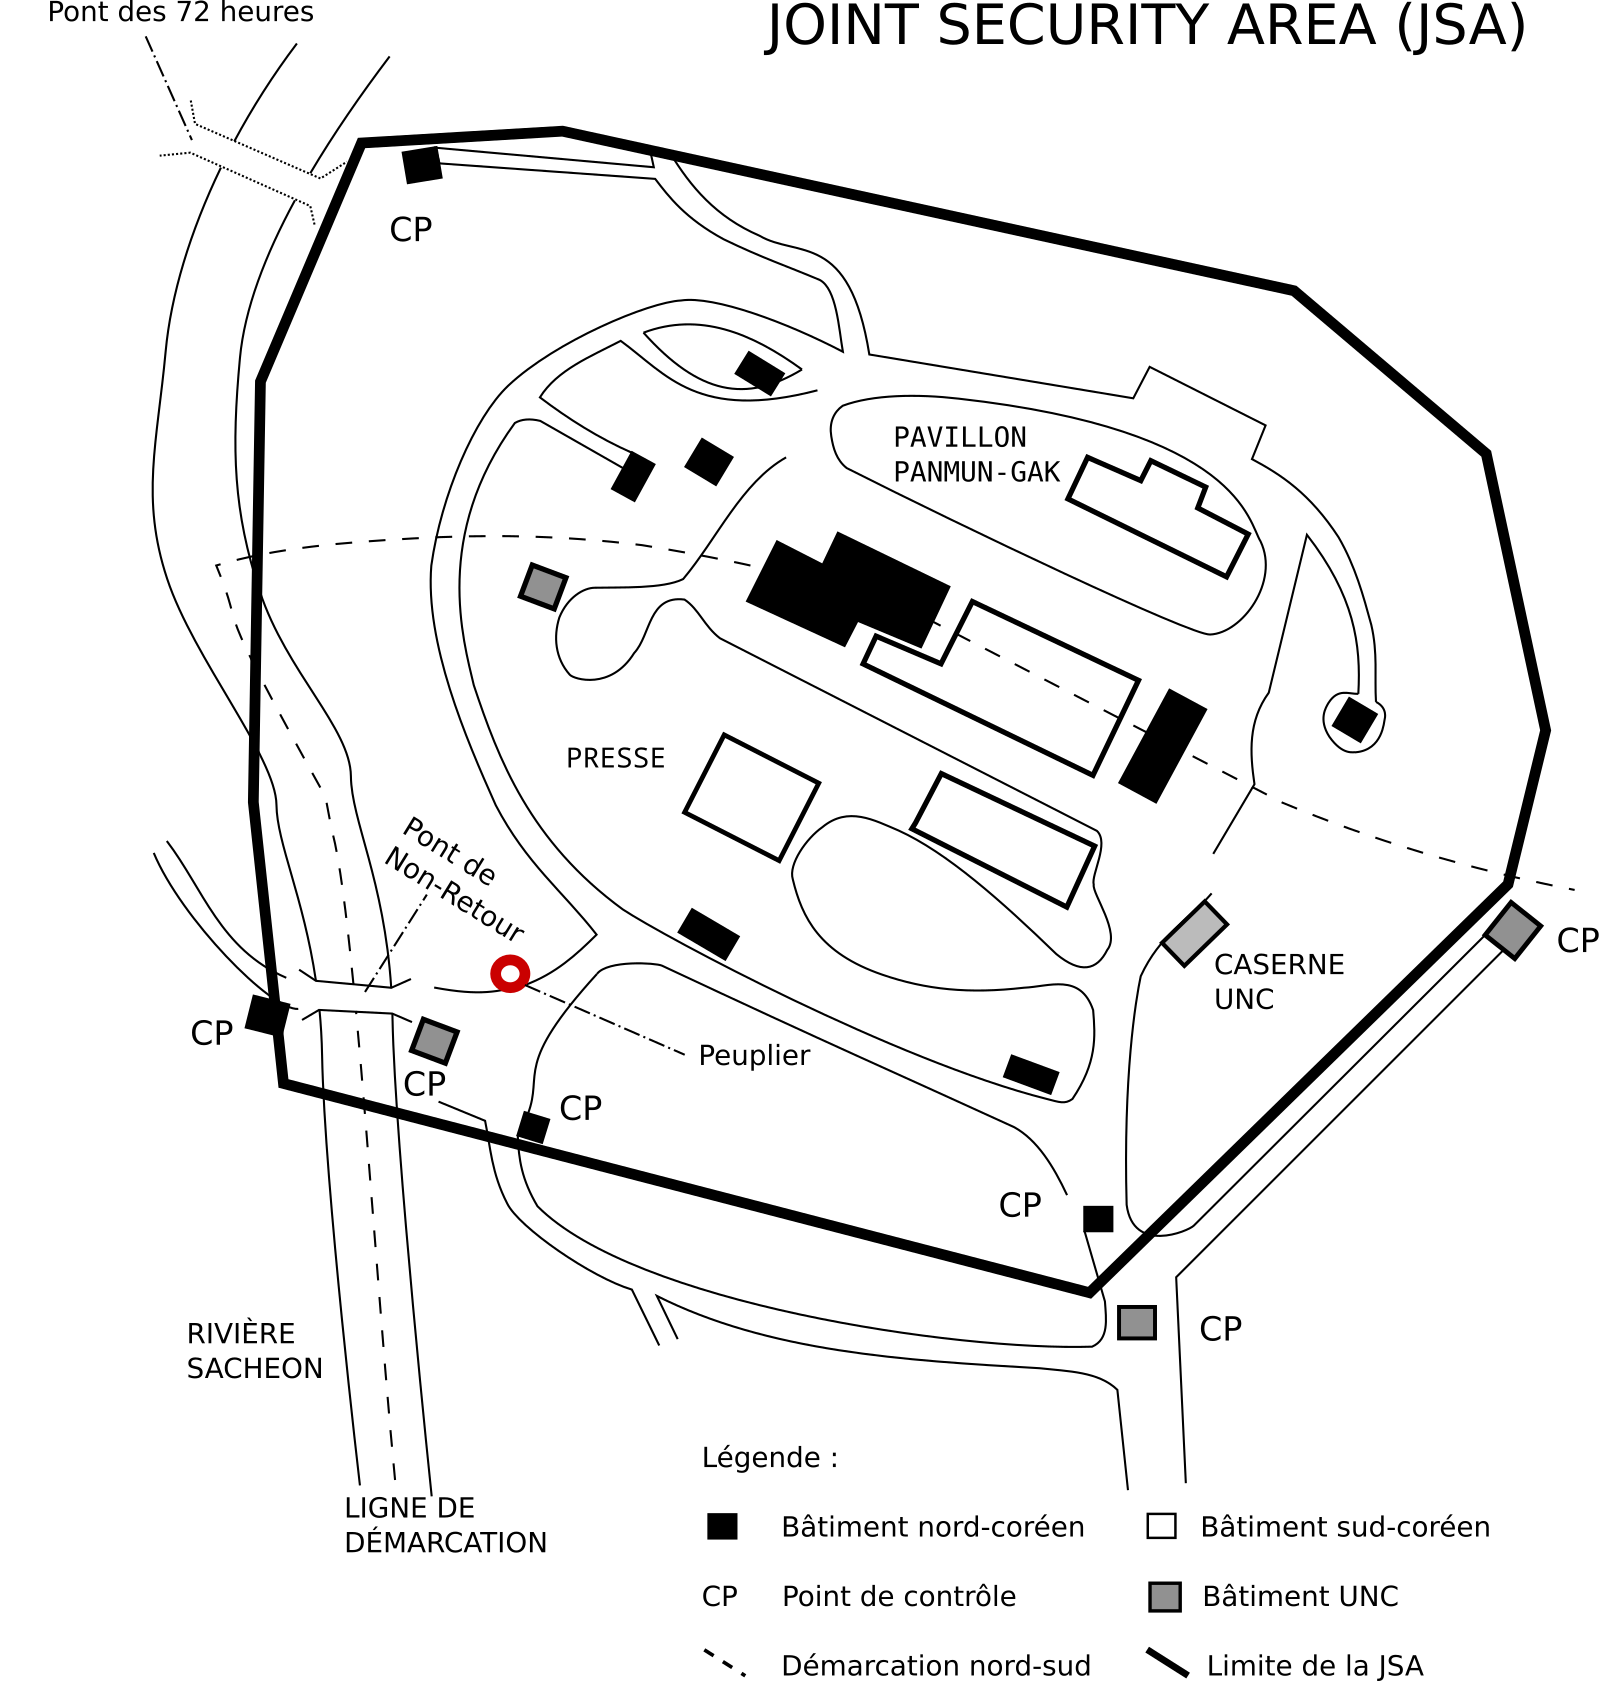
\includegraphics[width=\textwidth]{images/jsa.png}

\begin{tcolorbox}[colback=black!1!white]
La zone de sécurité commune se situe dans la zone démilitarisée entre les deux Corées.
L'endroit est sous contrôle simultané des deux pays et les personnels d'un camp comme de l'autre peuvent s'y déplacer librement.
Les forces sud-coréennes sont assistées par l'\emph{United Nations Command}, le commandement des Nations unies en Corée, installé par l'O.N.U. en 1950.

Le pont des 72 heures n'est pas encore construit au début du scénario. Il s'agit du pont que les nord-coréens construisent pour s'affranchir du pont de Non-Retour et qui leur permettra par la suite de traverser la rivière Sacheon sans passer par la JSA.
\end{tcolorbox}

\begin{table}
	\caption{Événements aléatoires durant l'abattage du peuplier}
	\label{table:peuplier}
	\colortablerows
	\begin{tabularx}{\textwidth}{cX}
	d8 & Événement\\
	1  & Les tronçonneuses tombent en panne après quelques minutes. Il faut soit en faire venir des nouvelles, soit finir le travail à la hache.\\
	2  & Un soldat américain s'avance sur le pont et provoque les nord-coréens. Il se trouve qu'il est proche d'un des officiers assassinés.\\
	3  & Des camions nord-coréens s'installent à 150m et construisent un nouveau pont.\\
	4  & Les nord-coréens font s'avancer les prisonniers sur le pont. Ils seront relâchés si les forces impérialistes renoncent, sinon ils seront exécutés.\\
	5  & Un des soldats sud-coréens se comporte étrangement. Il transmet discrètement des informations au régime du nord sur l'avancée de l'opération américaine.\\
	6  & Les renseignements japonais ont intercepté un message nord-coréens : leurs troupes s'apprêteraient à bloquer la rivière Imjin. C'est malheureusement la route prévue par le commandement de l'O.N.U. pour une évacuation par canots en cas d'attaque\dots\\
	7  & Un jeune nord-coréen saute dans la rivière et tente de traverser à la nage. Il appelle à l'aide en anglais et jure qu'il veut faire défection.\\
	8  & Alors que les sapeurs ramassent les branches déjà coupées et les chargent dans un pick-up conformément aux ordres, les sud-coréens leur demandent de les laisser sur place. Compte-tenu du symbolisme de l'arbre, les nord-coréens pourraient prendre cet acte pour une provocation.\\
	\end{tabularx}
\end{table}

\vfill
\illustration[\textwidth]{chainsaw}
\vfill
